\section{Background}
\label{sec:background}
This section gives the necessary background information about the technologies used in this work to build an AI agent.

\subsection{Agents and AI Agents}
// TODO

\subsubsection{Agent}
From a very basic perspective, an agent is an entity which is able to produce some effect or make changes in its
environment \parencite{CASTELFRANCHI1998157}.

\subsubsection{AI Agent}
\label{sec:AI_Agent}
With the rise of generative AI a new term "AI Agent" has emerged.
AI Agents can be defined as software entities which are designed to fulfill goal-oriented tasks.
Such agents can take in information from their environment, be it structured or unstructured inputs, draw conclusions from
the context and initiate actions toward achieving specific objectives. Rather than executing a
predetermined and deterministic sequence of steps like a traditional agent, an AI Agent can respond to what it observes while running,
adjusting its behaviour and the results it produces as the situation changes. The primary decision-making engine for these
AI Agents are LLMs (see \cref{sec:LLMs}) \parencite{Sapkota_2026}.



\subsection{Large Language Models (LLMs)}
\label{sec:LLMs}
Large Language Models (LLMs) are an evolution
 in artificial intelligence, moving from
 rule-based systems to general-purpose generative models. An LLM is essentially
 a complex statistical system designed to predict the likelihood of
 a sequence of words. By training on massive amounts of text, often
 using lots of data from the public internet. These
 models learn to generate coherent and contextually appropriate
 continuations for a given input prompt \parencite{douglas2023largelanguagemodels}.


\subsection{Tokens, Context Windows and Cost}
\label{sec:tokens-context-cost}
LLMs do not operate on text (words and characters) directly. Text has to first go through a \emph{tokenizer} that breaks it into pieces called \emph{tokens}
which can be words, sub-words or even just single characters. The goal of a \emph{tokenizer} is to return an efficient set of tokens to represent a text dataset. \parencite{alammar2024hands}

Each model can only process a limited number of tokens at once. This upper bound is referred to as the
\emph{context window} and covers the prompt, any provided tools, the conversation history and the generated
response. Beyond being a hard limit, longer contexts also degrade the quality of the model's output:
\textcite{liu-etal-2024-lost} show that models use information most reliably when it appears at the beginning or the
end of the context and perform noticeably worse when relevant information is located in the middle, a
phenomenon known as "lost in the middle". The degradation is not only a question of \emph{where} relevant
information sits, but also of \emph{how much} context surrounds it: \textcite{hong2025context} evaluate a
range of state-of-the-art models on deliberately simple tasks and find that performance declines, as the input grows longer, even when the task itself does not become harder. These two properties, the finite context window and the
degradation over long contexts, are a central motivation for distributing work across several specialised
agents rather than handling everything in a single, ever-growing context (see \cref{sec:multi-agent}).


\subsection{Multi-Agent (AI) Systems}
\label{sec:multi-agent}
A multi-agent (AI) systems (MAS) are systems composed of multiple interacting agents. 
MAS (Multi-agent systems) are able to solve more difficult problems compared to individual agents (a monolithic system) \parencite{tran2025multiagentcollaborationmechanismssurvey} 

With the rise of LLM-based agents (AI Agents) (see \cref{sec:LLMs}), this idea has been transferred to systems in which
the individual agents are driven by LLMs. \textcite{tran2025multiagentcollaborationmechanismssurvey} work describes how
multiple LLM agents collaborate through different coordination structures. This work uses a \emph{hierarchical} structure together with
a \emph{role-based} collaboration strategy. A detailed view of the architecture in this work is described in \cref{sec:concepts}.

Splitting a task across several specialised agents has practical benefits that follow directly from the
limitations discussed in \cref{sec:tokens-context-cost}: each agent can be given a focused instruction set and
a smaller selection of tools, which keeps its individual context small, reduces the risk of context-related
quality degradation.




\subsection{Function Calling}
\label{sec:func-calling}
LLMs have great generative capabilities but they lack the ability to perform any task beyond generating a response.
This means LLMs are not able to retrieve any external information in real time. 
This limitation means LLMs only have access to the static training data, this inherently results in reponses that are plausible but factually incorrect or outdated (often referred to
as hallucination). \parencite{Qu_2025}. 
To address this limitation a paradigm named "Function Calling" has been developed. 
It solves these problems by giving LLMs the ability to interact with external systems by invoking predefined blocks of code (functions) \parencite{wang2026FunctionCalling}.

\subsubsection{Function Calling process example using OpenAI API}
The following Image illustrates the function calling principle using the OpenAI function calling API as an example. The function calling API is an optional part of the new \emph{Responses API} or the older \emph{Chat Completions API} \parencite{openai_responses_create}.

\begin{enumerate}
    \setlength{\itemsep}{8pt}
    \item The prompt message and all the tool definitions are sent to the model.
    \item Based on the provided prompt and tools the model decides to call some function, providing the necessary arguments (in this example "paris").
    \item The function chosen by the model is executed.
    \item All prior messages together with the result (output) of the function execution are sent back to the model.
    \item Based on all the messages the model gives back a final response \parencite{openai_function_calling}.
\end{enumerate}

\begin{figure}[htbp]
\begin{center}
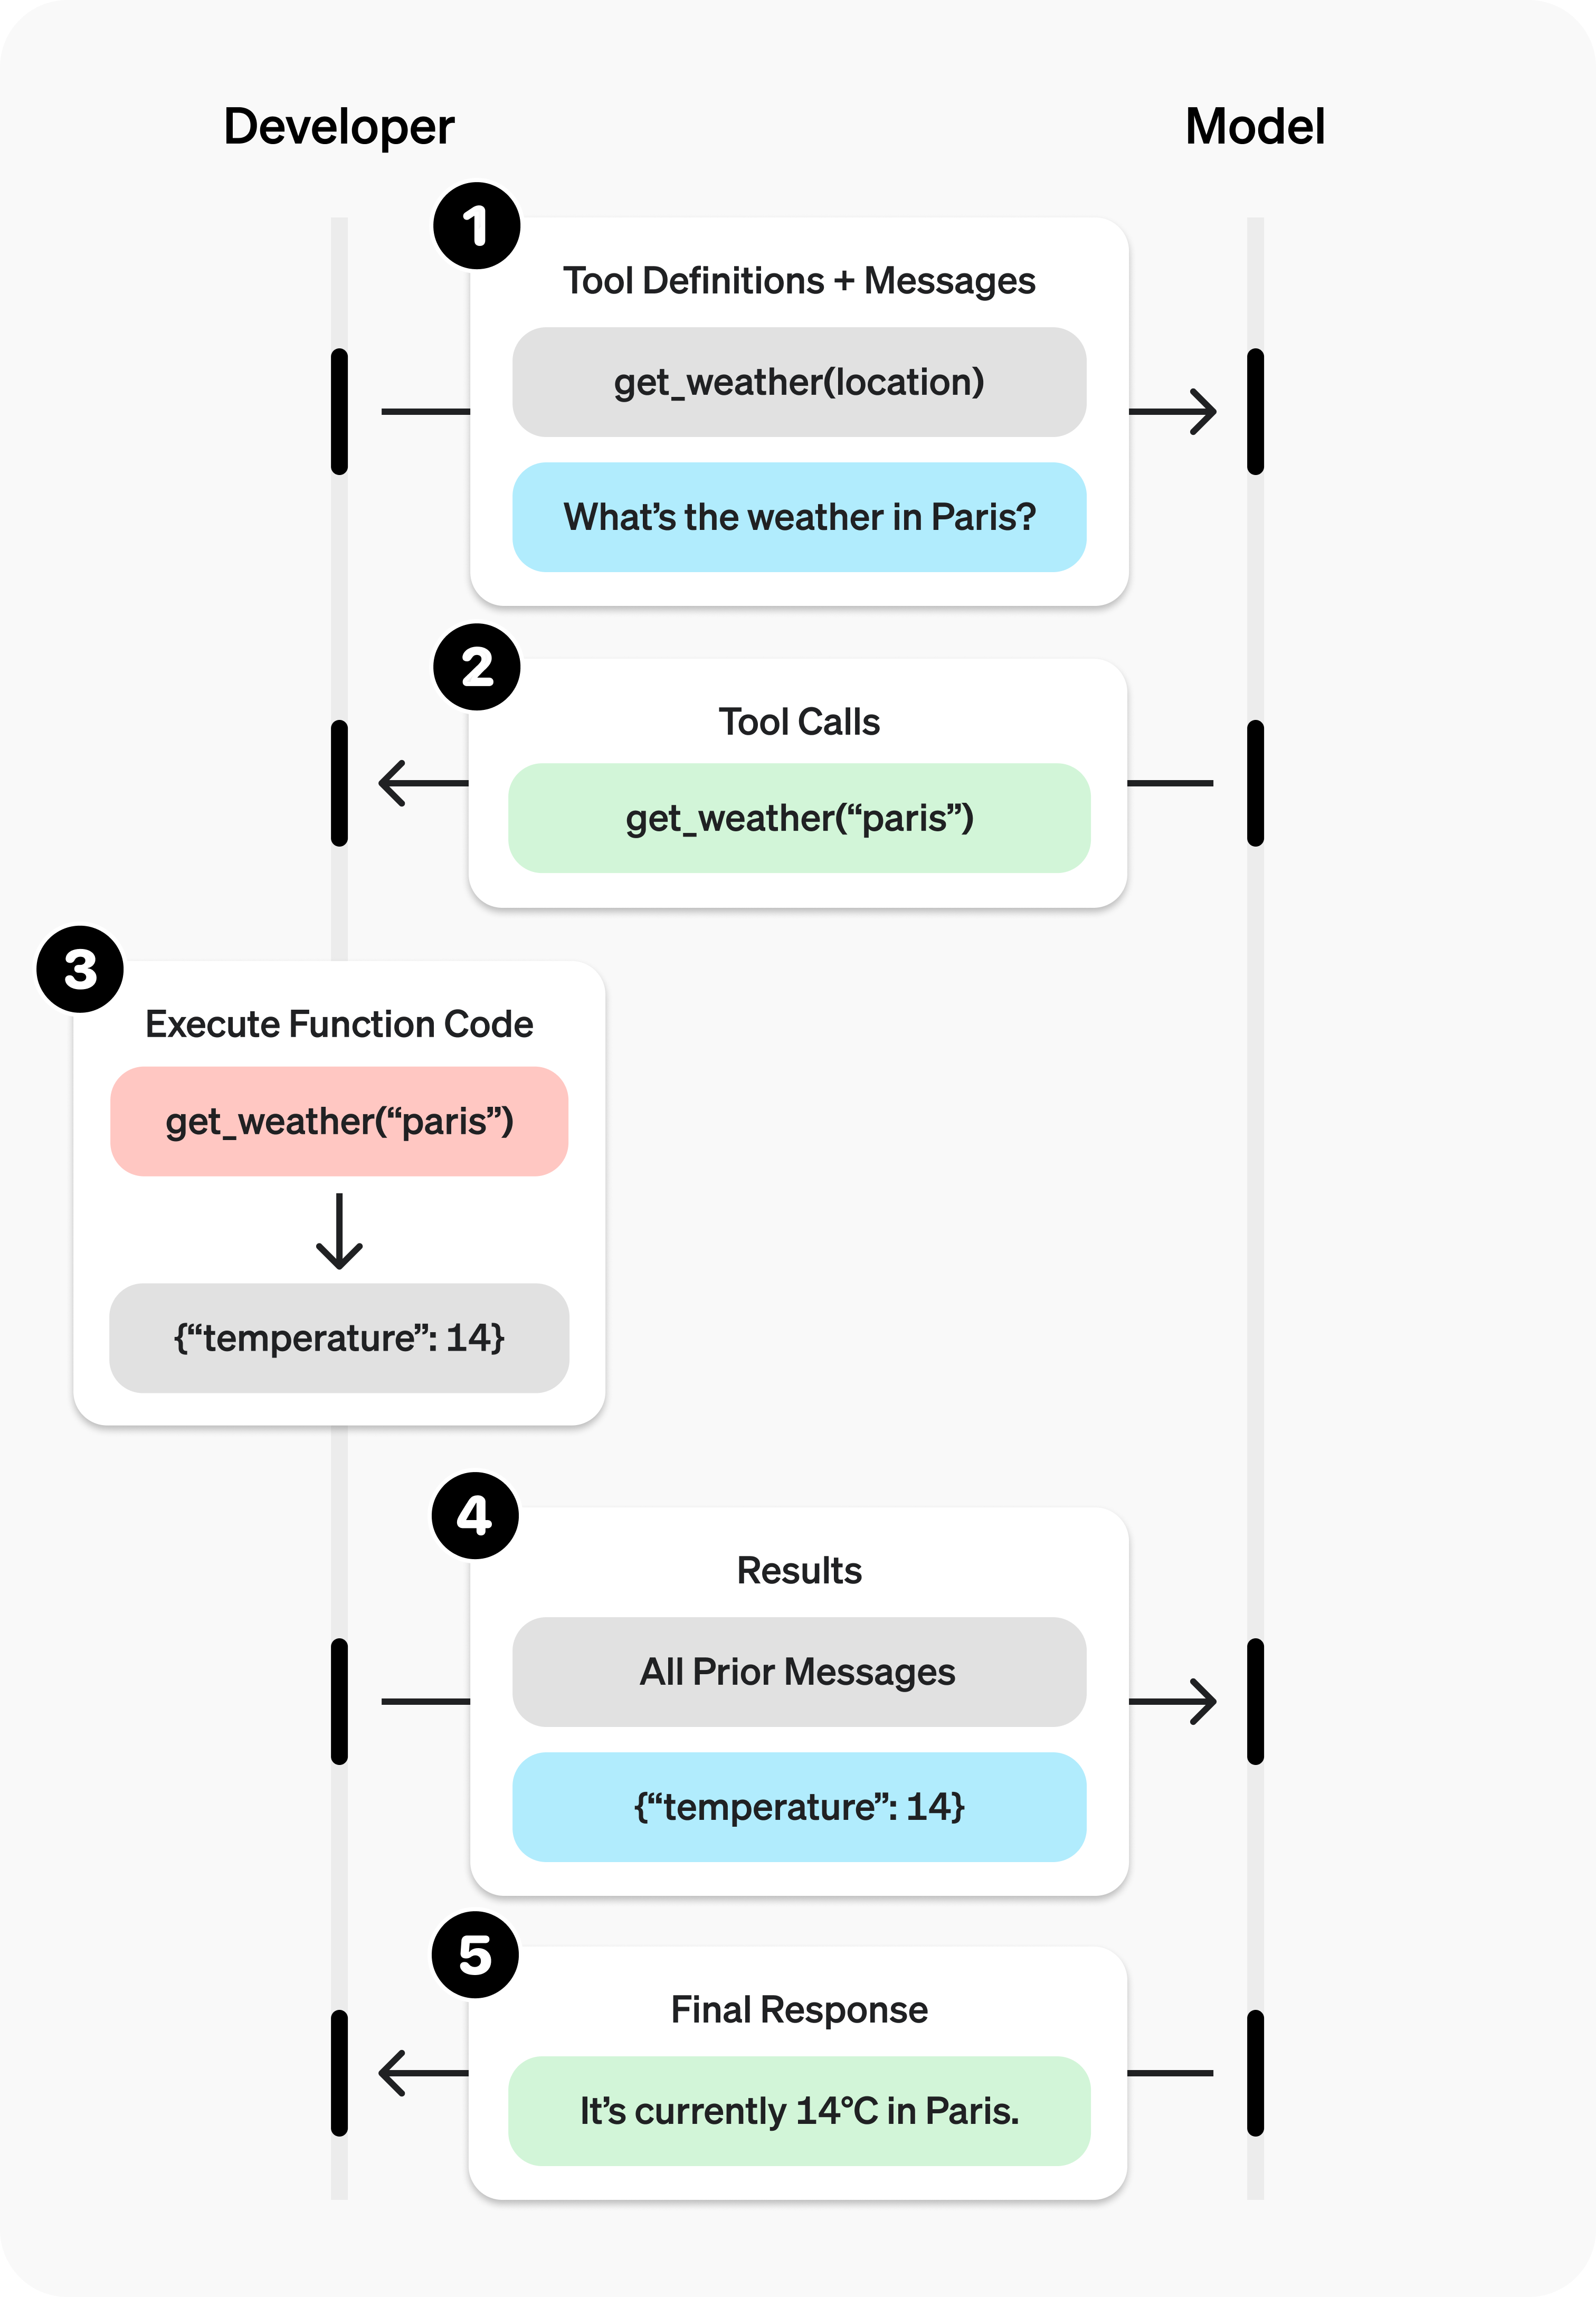
\includegraphics[width=0.9\linewidth]{graphics/function-calling-diagram-steps.png}
\end{center}
\caption{Function calling procedure
\parencite{openai_function_calling}}
\label{fig:function-calling-procedure}
\end{figure}

\newpage
\subsection{Agent Loop and Agent Harness}
\label{sec:agent-loop}

\subsubsection{Agent Loop}
Function calling (see \cref{sec:func-calling}) describes a \emph{single} exchange in which the model receives a function, requests a
function execution and receives its result. On its own, this does not yet make a system agentic. The model still needs to be
invoked repeatedly, decide when another tool call is necessary, and recognise when the task is complete. This
repetition is captured by the term \emph{agent loop}, the core control cycle of an AI Agent. The model receives the current
context, decides on an action (either calling a tool or producing a final answer), the chosen tool is executed, its
result is appended to the context, and the cycle repeats until the model returns a final answer or a stop condition is
reached \parencite{yao2023reactsynergizingreasoningacting,anthropic_effective_agents,strands_agent_loop}. These steps of reasoning and acting were introduced
as the \emph{ReAct} pattern by \textcite{yao2023reactsynergizingreasoningacting}. The agent loop is therefore what elevates a sequence of isolated
function calls into goal-oriented behaviour that adapts to what the model observes while running, as introduced in
\cref{sec:AI_Agent}.

\Cref{fig:agent-loop} shows this cycle: an initial input and context enter the loop, the model reasons and selects a
tool, the tool is executed and its result is fed back for the next round of reasoning, and the loop repeats until the
model produces a final response.

\begin{figure}[htbp]
\begin{center}
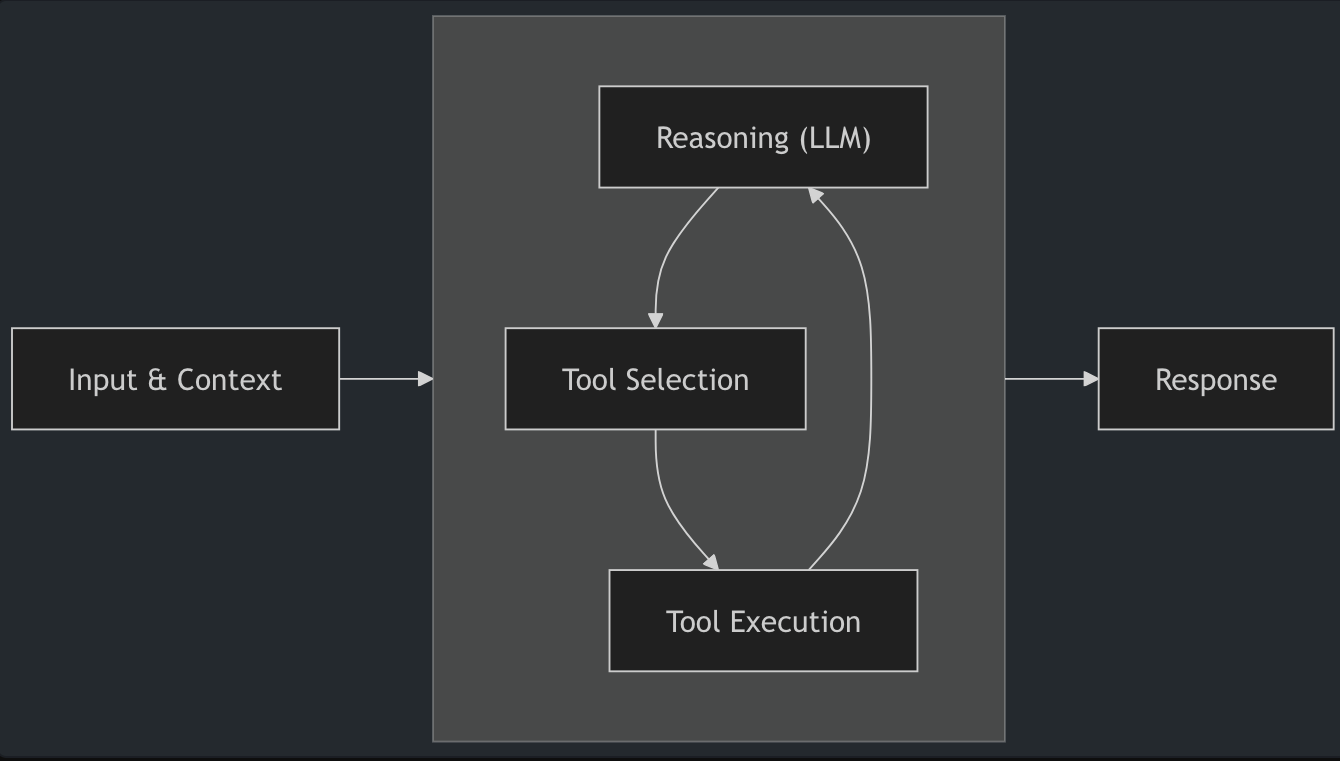
\includegraphics[width=0.9\linewidth]{graphics/agent-loop-strandsagents.png}
\end{center}
\caption{The agent loop \parencite{strands_agent_loop}}
\label{fig:agent-loop}
\end{figure}
\newpage

\subsubsection{Agent Harness}
An LLM by itself cannot run this loop (agent loop), it only predicts a single continuation for a given input
(see \cref{sec:func-calling}). The loop, the dispatching of tool calls, the accumulation of the message history and the
evaluation of stop conditions all have to be implemented by the surrounding software. This runtime software is
commonly referred to as the \emph{agent harness}, the software infrastructure that wraps around an LLM and enables it to
act on tasks rather than only respond to prompts, often summarised as \emph{Agent = Model + Harness}
\parencite{databricks_ai_harness,langchain_agent_harness}. The harness is the engine that drives the agent loop (the core) and manages the
things around it. It forwards the conversation and the available tool definitions to the model, executes the tool
calls the model requests and maintains the message history across iterations. In practice a
harness is most of the time provided by an \emph{agent framework} with APIs to modify and add additoanl functionalities. The concrete framework used in this work is described in
\cref{sec:implementation}.

\Cref{fig:agent-harness} illustrates this relationship: the model sits at the centre and only reasons and decides,
while everything around it, the context injection, control, action (tool calls), observation and persistence, is
provided by the surrounding harness.

\begin{figure}[htbp]
\begin{center}
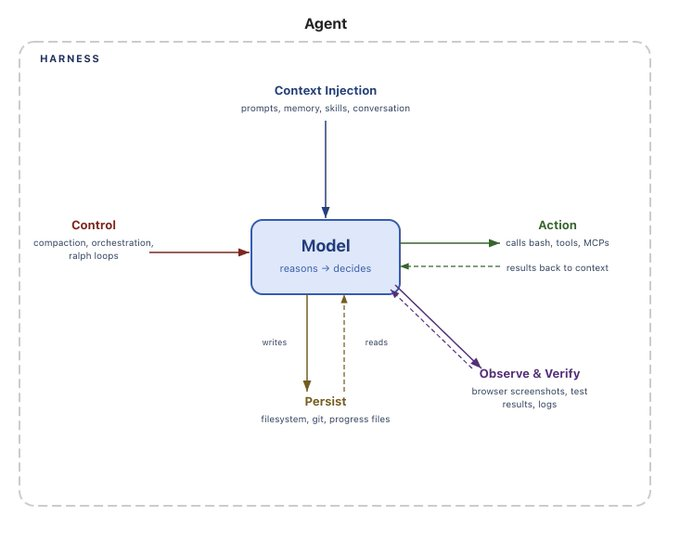
\includegraphics[width=0.9\linewidth]{graphics/langchain-anatomy-of-an-agent-harness.png}
\end{center}
\caption{Anatomy of an agent: the model surrounded by the harness
\parencite{langchain_agent_harness}}
\label{fig:agent-harness}
\end{figure}


\newpage
\subsection{Model Context Protocol (MCP)}
\label{sec:mcp}
The Model Context Protocol (MCP) is an open-source standard designed to facilitate the connection between AI
 applications and external systems. MCP allows AI models (such as ChatGPT) to securely interact with different
 data sources (like local files and databases) and tools (execute functions).

The core problem MCP addresses is the fragmentation of AI integrations. Before MCP, every
new data source required its own custom implementation, making truly connected systems
difficult to scale \parencite{mcp_anthropic}. This is commonly framed as the $N \times M$
integration problem \parencite{mcp_nxm}. Without a common standard, connecting $N$ AI
applications to $M$ external systems (data sources and tools) requires a custom 
integration for every AI-Application, external system pair, resulting in up to $N \times M$ separate
integrations that must each be built and maintained individually. MCP replaces this with a
single shared protocol. Every AI application implements the MCP client side once, and every
external system is exposed through an MCP server once. This reduces the integration effort
from a multiplicative $N \times M$ to an additive $N + M$. 
\parencite{mcp_nxm}.

As illustrated in \cref{fig:mcp_architecture-overview}, MCP therefore functions similarly to a
"USB-C port for AI applications," providing a standardized way to connect AI
applications to external systems \parencite{mcp_intro}.

\begin{figure}[htbp]
\begin{center}
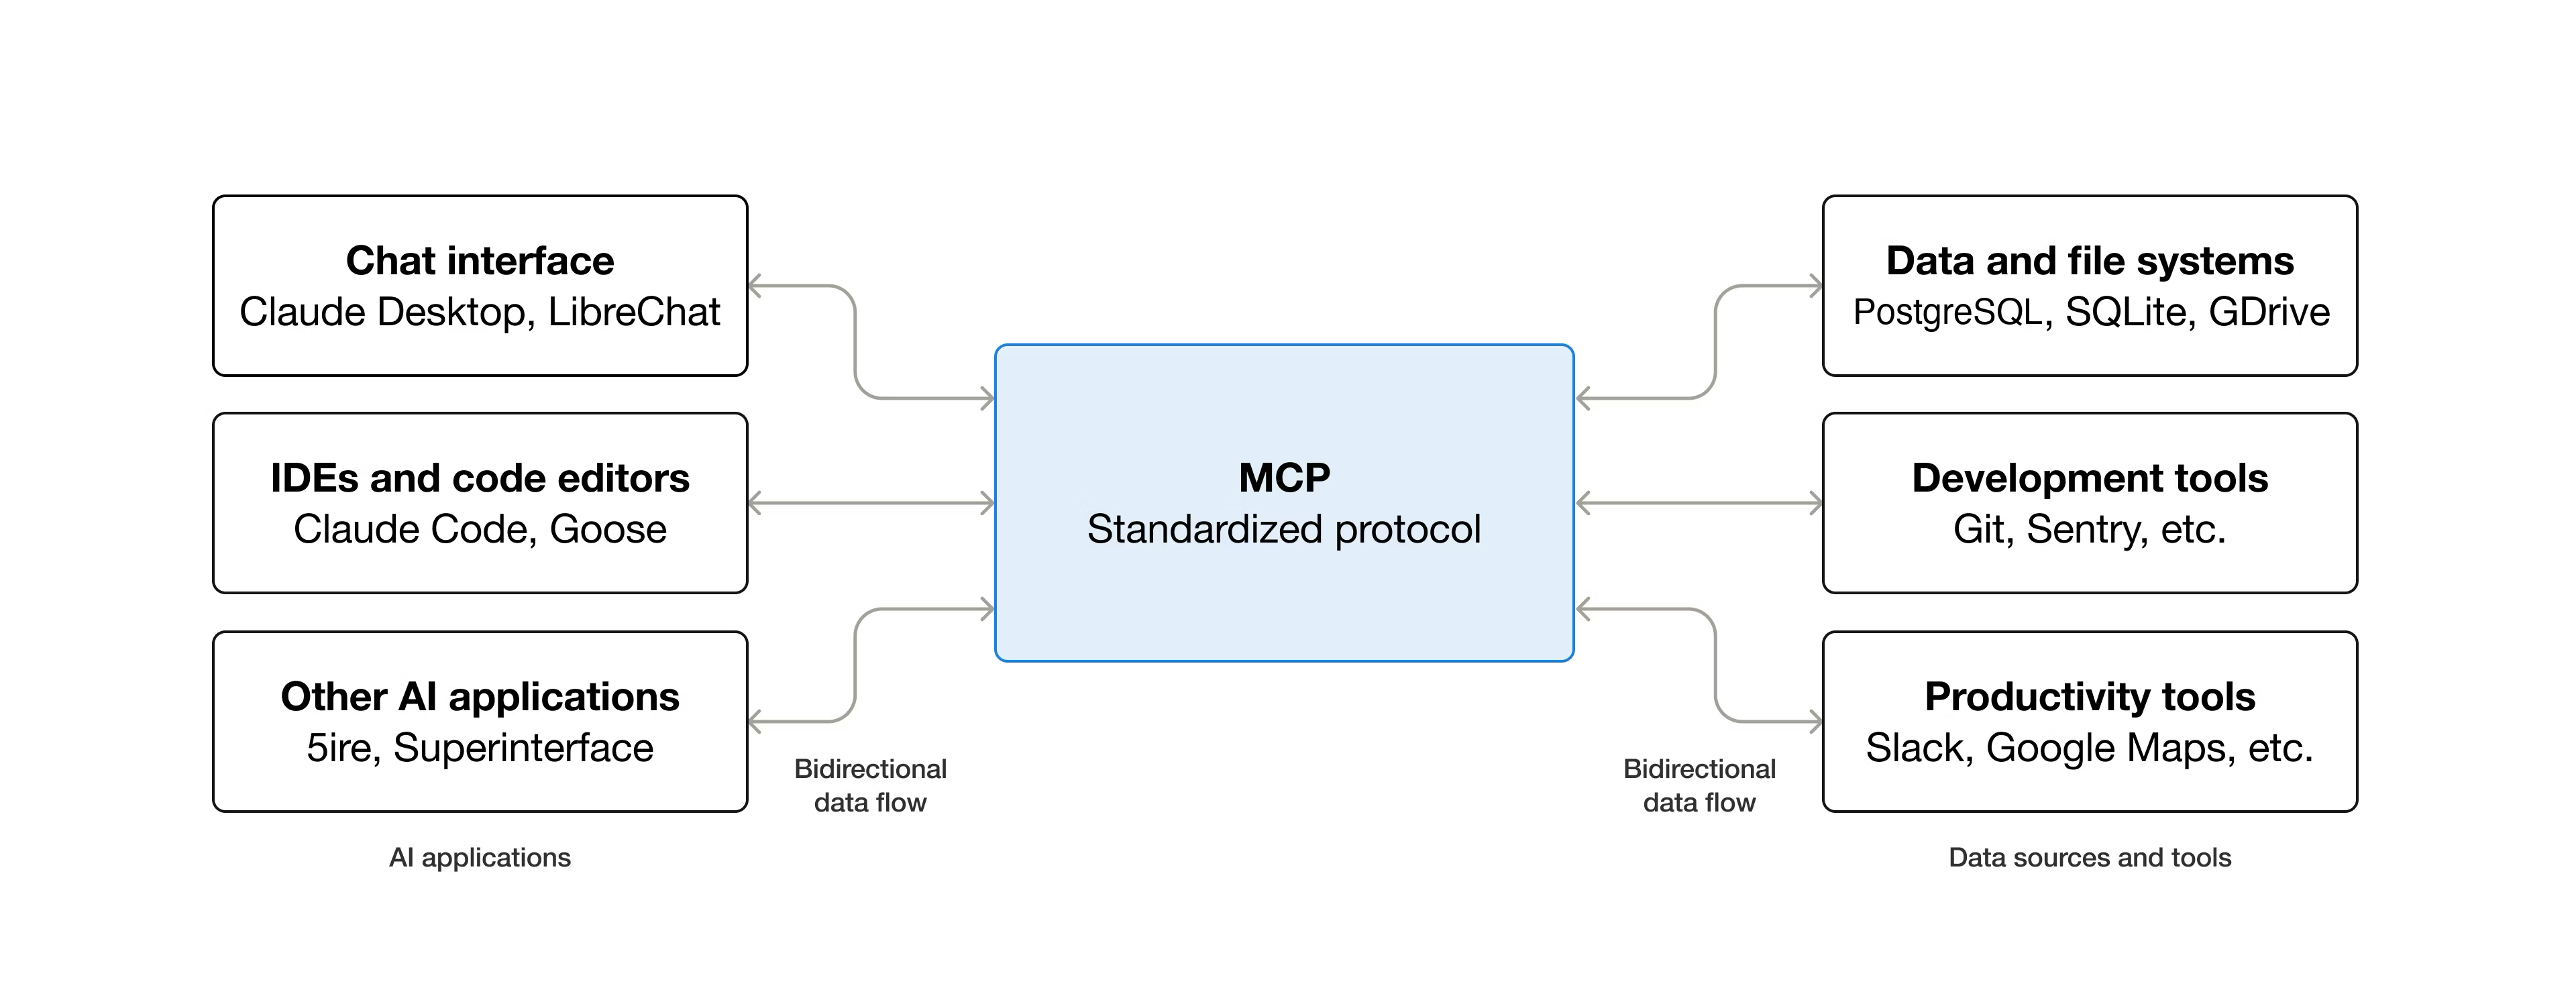
\includegraphics[width=0.9\linewidth]{graphics/mcp-architecture-overview.png}
\end{center}
\caption{MCP architecture
\parencite{mcp_intro}}
\label{fig:mcp_architecture-overview}
\end{figure}






